\chapter{Eksperyment LHCb}

Ten rozdział opisuje pokrótce eksperyment LHCb. Na samym początku omówione zostanie fundamentalne prawo fizyki łączące zasady zachowania z~ symetriami. Następnie opisane zostaną dyskretne symetrie w kontekście najnowszych badań doświadczalnych.   

\section{Symetrie w fizyce}
Jeżeli chce się mówić na temat fizyki zawsze powinno się zacząć od tematu symetrii. Jedną z~ najbardziej fundamentalnych zasad w~ fizyce jest ta, łącząca prawa zachowania z~ symetriami natury. Twierdzenie Noether \cite{Noether} pokazuje, że jeśli układ fizyczny jest niezmienniczy \footnote{rozumiemy tu Lagranżjan opisujący ten układ} względem pewnej ciągłej transformacji,to istnieje prawo zachowania wielkości stowarzyszonej z~ tą transformacją. Niezmienniczość praw fizycznych względem translacji czasowej jest odpowiedzialna za istnienie fizycznej zasady zachowania energii. Zasada zachowania pędu jest konsekwencją niezmienniczości względem przesunięć w przestrzeni. Natomiast zasada zachowania momentu pędu jest spełniona gdy prawa fizyki są identyczne po uwzględnieniu obrotów w przestrzeni. 

Poza wyżej wymienionymi symetriami ciągłymi istnieją jeszcze symetrie dyskretne tzw. punktowe. Z~ punktu widzenia fizyki cząstek elementarnych istotnymi symetriami są:

\begin{itemize}
\item \textbf{$\hat{C}$}- sprzężenie ładunkowe (ang. charge conjugation) zmienia znak wszystkich addytywnych liczb kwantowych danej cząstki. W specyficznym odniesieniu do rozpadów sub-atomowych cząstek, sprzężenie ładunkowe oznacza zamianę każdej cząstki na sprzężoną z nią antycząstkę.\cite{symmetry}.
\item \textbf{$\hat{P}$}- parzystość (ang. parity) jest to operacja zamiany wszystkich współrzędnych przestrzennych na przeciwne. \cite{symmetry}
\item \textbf{$\hat{T}$} odwrócenie czasu (ang. time reversal) zmienia kierunek przepływu czasu na przeciwny \cite{symmetry}.
\end{itemize}

Według obecnej wiedzy, każda z tych symetrii jest zachowana w oddziaływaniach silnych i~ elektromagnetycznych. Natomiast, co bardziej interesujące, słabe oddziaływania łamią symetrie \textbf{$\hat{C}$} oraz  \textbf{$\hat{P}$}. Jednakże, kombinacja tych symetrii \textbf{CPT} jest dokładną symetrią w każdej lokalnej Lorentz'ko niezmienniczej teorii pola \cite{symmetry}.

\section{Symetrie a początek Wszechświata}
W przybliżeniu po okresie $10^{-6}s$ do Wielkiego Wybuchu została uformowana plazma kwarkowo-gluonowa w której to wolne kwarki oraz gluony podróżowały z relatywistycznymi prędkościami. Pary cząstka-antycząstka były stale tworzone oraz anihilowane, tworząc fotony, równomiernie poruszające się przez kosmos. Po tym procesie, do dzisiaj pozostało tzw. Mikrofalowe Promieniowanie Tła (ang. \textbf{C}osmic \textbf{M}icrowave \textbf{B}ackground). Na podstawie badań tego promieniowania oszacowano wiek Wszechświata na $13.75 \pm 0.11$ miliarda lat \cite{CMB}.

Niedługo, po tym jak CMB zostało wytworzone jedna z liczb kwantowych \textit{liczba barionowa} została złamana, w wyniku czego ilość produkowanych cząstek była większa niż ilość wytwarzanych antycząstek. Ten proces nazywany \textit{bariogenezą} tłumaczy niewystępowanie antymaterii w~ obecnym wszechświecie. Co, oczywiście prowadzi do prostego wniosku - dzisiejszy wszechświat zbudowany jest z~ materii.

W 1967 Sacharow  wyjaśnił \cite{Sacharow}, istnienie Wszechświata w obecnej formie wymaga spełnienienia trzech warunków.
\begin{enumerate}
\item Niezachowania liczby barionowej. 
\item Ochładzanie Wszechświata zachodziło w warunkach niebędących w równowadze termodynamicznej. 
\item Zachodzenie procesu łamania symetrii kombinowanej \textbf{CP} 
\end{enumerate}

\section{Symetria kombinowana \textbf{CP}}
Symetria kombinowana \textbf{CP}, będąca jak uprzednio wspomniano jednym z warunków Sacharowa do tego, aby istniał wszechświat, była poddana obserwacji już wcześniej. Powodem tego było odkryciem istnienia tylko lewoskrętnych\footnote{Skrętność oznacza rzut wektora spinu na kierunek ruchu cząstki} neutrin i prawoskrętnych antyneutrin. Wynikiem zastosowania operatora \textbf{CP}\footnote{Operatory \textbf{C} oraz \textbf{P} komutują ze sobą nawzajem} na neutrino lewoskrętne jest antyneutrino prawoskrętne. Stąd sądzono, że ta symetria jest zachowana przez oddziaływania słabe. Obrazowo działania tych operatorów zostały zaprezentowane na rysunku \ref{fig:CP}.


 \begin{figure}[ht]
 \centering
 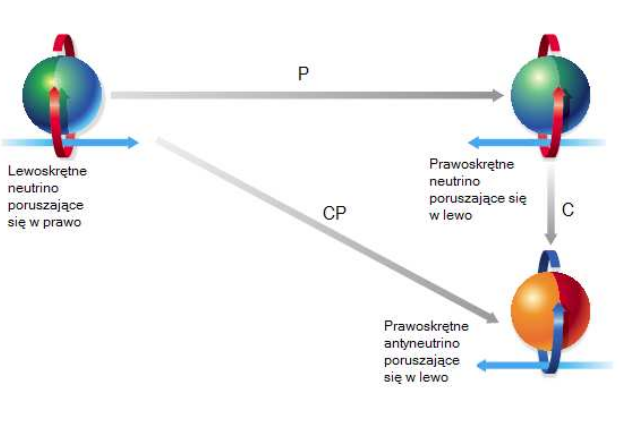
\includegraphics[scale=0.5]{rozdzial1/CP.png}
 % Beetle_block.jpeg: 848x489 pixel, 96dpi, 22.44x12.94 cm, bb=0 0 636 367
 \caption{Działanie operatorów C, P i CP na neutrino}
 \label{fig:CP}
\end{figure}


 Tak było do roku 1964, kiedy to rozpad neutralnych kaonów pokazał, że ta symetria jednak jest łamana. Pierwszym dowodem na łamanie  \textbf{CP} poza układem kaonów, został zaobserwowany w 2001 roku przez eksperyment Belle. Obiektami ich badań były układy neutralnych mezonów B\footnote{Mezon B to hadron składający się z kwarka b oraz lżejszego antykwarka } . Odkrycie zapoczątkowało nową erę badań procesów łamiących symetrię  \textbf{CP}. Lekkie mezony B (neutralne $B_u$ oraz naładowane $B_d$ były poddawane precyzyjnym pomiarom przez fabryki-B: Belle oraz BaBar. LHCb jest eksperymentem drugiej generacji. Jego krótki opis umieszczono w~  rozdziale 2.
\subsection{Teoretyczny opis łamania symetrii \textbf{CP} }

Stany własne oddziaływań słabych nie są tożsame ze stanami własnymi oddziaływań silnych\footnote{zwane również stanami własnymi masy}. Przejście z~ jednej bazy do drugiej możliwe jest dzięki macierzy Cabbibo-Kobayashi-Maskawy (CKM).
\begin{equation}
\begin{pmatrix}
d'\\ s' \\b'
\end{pmatrix} =V_{CKM} 
\begin{pmatrix}
d\\ s \\b
\end{pmatrix}=\begin{pmatrix}
V_{ud}& V_{us}&V_{ub}\\ V_{cd}& V_{cs}&V_{cb} \\ V_{td}& V_{ts}&V_{tb}
\end{pmatrix} \begin{pmatrix}
d\\ s \\b
\end{pmatrix}
\end{equation}

Macierz CKM jest macierzą unitarną trzeciego rzędu. Rozmiar macierzy odpowiada ilość rodzin kwarkowych. Zostało udowodnione\footnote{na podstawie pomiarów astronomicznych oraz niezależnie eksperymentu DELPHI\cite{delphi} }, że istnieją tylko 3 rodziny. Elementy macierzy określają stałe sprzężenie pomiędzy odpowiednimi kwarkami. Warto zwrócić uwagę, że Model Standardowy w~ żaden sposób nie przewiduje wartości elementów macierzy CKM. Wartości te należy wyznaczyć doświadczalnie. 

W ciągu wielu lat teoretycznych studiów nad macierzą CKM teoretycy zaproponowali kilka sposobów jej parametryzacji. Do najbardziej uznanych należy parametryzacja Keung-Chau, zwana również standardowa. 
\begin{eqnarray}
V_{CKM}&=&\begin{pmatrix} 1 & 0 & 0 \\ 0 & c_{23} & s_{23} \\ 0 & -s_{23} & c_{23} \end{pmatrix}
 \begin{pmatrix} c_{13} & 0 & s_{13}e^{-i\delta_{13}} \\ 0 & 1 & 0 \\ -s_{13}e^{i\delta_{13}} & 0 & c_{13} \end{pmatrix}
 \begin{pmatrix} c_{12} & s_{12} & 0 \\ -s_{12} & c_{12} & 0 \\ 0 & 0 & 1 \end{pmatrix} \nonumber \\
V_{CKM}&=&\begin{pmatrix}
c_{12}c_{13}&s_{12}c_{13}& s_{13}e^{-i\delta} \\
 -s_{12}c_{23}-c_{12}s_{23}s_{13}e^{i\delta} & c_{12}c_{23}-s_{12}s_{23}s_{13}e^{i\delta}  & s_{23}c_{13}\\ s_{12}s_{23}-c_{12}c_{23}s_{13}e^{i\delta} & -c_{12}s_{23}-s_{12}c_{23}s_{13}e^{i\delta} & c_{23}c_{13}
\end{pmatrix}
\end{eqnarray}

gdzie:\\
$c_{ij}=cos\theta_{ij}$ oraz $s_{ij}=sin\theta_{ij}$. Warte wyjaśnienie jest znaczenie kąta $\theta_{ij}$ oraz $\delta$. $\theta_{ij}$ są to tzw. katy Eulera\footnote{Układ trzech kątów, za pomocą których można jednoznacznie określić wzajemną orientację dwóch układów współrzędnych.} mówiące o~ stopniu mieszania pomiędzy trzema zapachami kwarków (i,j=1,2,3) oraz $\delta$ jest fazą odpowiedzialną za łamanie symetrii \textbf{CP}.

Ważną, z~ punktu widzenia hierarchizacji wielkości mieszanie pomiędzy rodzinami kwarkowymi jest tak zwana parametryzacja Wolfensteina \cite{Wolfenstein}. Każdy z~ elementów macierzy CKM jest wyrażany przez szereg potęgowy parametru $\lambda=sin\theta_{12}\approx 0.22$ . Kąt $\theta_{12}$ zwany jest kątem Cabibbo \citep{perkins}.

\begin{equation}
V_{CKM}=\begin{pmatrix}
1-\frac{1}{2}\lambda^2& \lambda & A\lambda^3(\rho-i\eta)\\
-\lambda & 1-\frac{1}{2}\lambda^2 & A\lambda^2\\
 A\lambda^3(\rho-i\eta) & -A\lambda^2 & 1
\end{pmatrix} +\mathcal{O}(\lambda^4) 
\label{Wolfenstein}
\end{equation}

Pozostałe parametry występujące w równaniu \ref{Wolfenstein} określone są zależnościami:
\begin{center}
\begin{tabular}{l c r}
$A \equiv \frac{s_{23}}{s^2_{12}},$&  $\rho \equiv  \frac{s_{13}cos\delta}{s_{12}s_{23}},$ & $\eta  \equiv \frac{s_{13}sin\delta}{s_{12}s_{23}}$
\end{tabular}
\end{center}

Ponieważ parametr $\lambda$ jest mniejszy od jedności to można, analizując wykładnik napisać względne relacje między poszczególnymi elementami macierzy CKM. Łatwo zauważyć, iż najbardziej prawdopodobne są przejścia między kwarkami tej samej rodziny.
\subsection{Trójkąty unitarności}

Wymogiem Modelu Standardowego jest unitarność macierzy CKM oznacza to, że musi zachodzić zależność
\begin{equation}
V^{\dagger}_{CKM}V_{CKM}=\mathbf{1}
\end{equation}
Z powyższego faktu wynika sześć warunków ortogonalności.
\begin{eqnarray}
db&:&V_{ud}V^*_{ub}+V_{cd}V^*_{cb}+V_{td}V^*_{tb}=0 \label{db} \\
sb&:&V_{us}V^*_{ud}+V_{cs}V^*_{cd}+V_{ts}V^*_{td}=0  \\
ds&:&V_{us}V^*_{ub}+V_{cs}V^*_{cb}+V_{ts}V^*_{tb}=0  \\
ut&:&V_{du}V^*_{dc}+V_{su}V^*_{sc}+V_{bu}V^*_{bc}=0  \\
ct&:&V_{dc}V^*_{dt}+V_{sc}V^*_{st}+V_{bc}V^*_{bt}=0  \\
uc&:&V_{dt}V^*_{du}+V_{st}V^*_{su}+V_{bt}V^*_{bu}=0  
\end{eqnarray}


Łatwo się przekonać, że każdy z powyższych warunków prowadzi do zanikania sumy trzech zespolonych liczb. Warunki unitarności mogą być przedstawione w postaci trójkątów w przestrzeni zespolonej (diagram Arganda) i~ nazywane są trójkątami unitarności. Każdy, z~ tych trójkątów posiada jednakowe pole, które można wyrazić, w~ notacji parametryzacji Wolfensteina, $P=\lambda^6A^2 \eta$.Trójkąty te wyróżnia długości ich boków.   Zaletą korzystania z~ formalizmu trójkątów unitarności jest fakt, że przy jakiekolwiek zmianie paramteryzacji macierzy CKM trójkąty zostają tylko obrócone w przestrzeni zespolonej natomiast długości boków oraz kąty pozostają bez zmian. 
 
 \begin{figure}[ht]
 \centering
 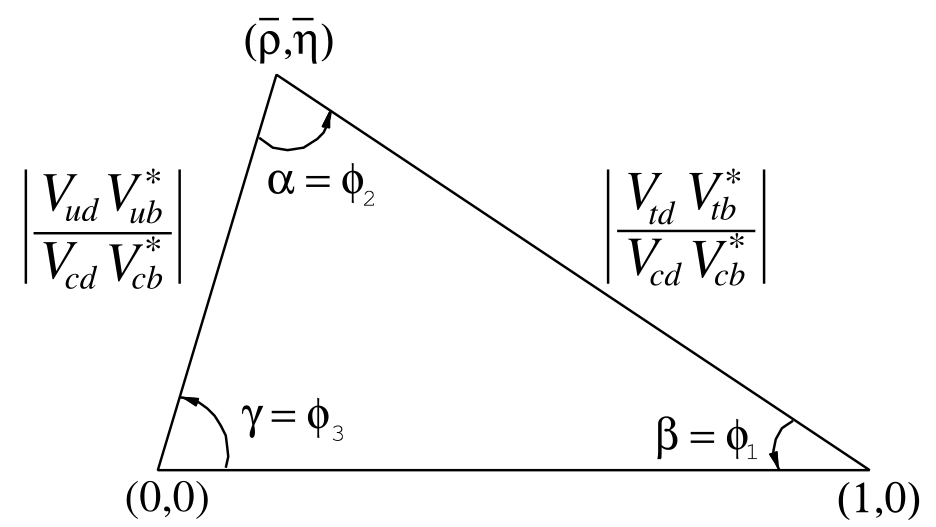
\includegraphics[scale=0.3]{rozdzial1/trojkat.png}
 % Beetle_block.jpeg: 848x489 pixel, 96dpi, 22.44x12.94 cm, bb=0 0 636 367
 \caption{Trójkąt unitarności, kąty $ \phi_{1,2,3}$} odpowiadają kątom $\alpha,\beta,\gamma$ w notacji używanej przez eksperyment BELLE. Dolny bok trójkąta posiada jednostkową długość jest to zgodne z przyjętą konwencją. \cite{PDG}
 \label{fig:trojkat db}
\end{figure}
 

Z eksperymentalnego punktu widzenia, najciekawszym trójkątem jest \ref{db} , ponieważ jego boki są porównywalnych rozmiarów co oznacza, że wszystkie kąty (bądź odpowiadające im fazy) są duże. Trójkąt przedstawiony jest na rysunku \ref{fig:trojkat db}. Użyto standardowego oznaczenia kątów ($\alpha , \beta , \gamma $), te trzy kąty odnoszą się do zespolonych komponentów macierzy CKM przez związki:

\begin{eqnarray}
\alpha &=& \arg \left(- \frac{V_{td}V^*_{tb}}{ V_{ud}V_{ub}^* }  \right) =\arg \left( \frac{(1-\frac{1}{2} \lambda^2)(i \eta -\rho )}{1-\rho -i\eta}  \right)\\
\beta &=& \arg \left(- \frac{V_{cd}V^*_{cb}}{ V_{td}V_{tb}^* }  \right) =\arg \left( \frac{1}{1-\rho -i\eta}  \right)\\
\gamma &=& \arg \left(- \frac{V_{ud}V^*_{cb}}{ V_{cd}V_{cb}^* }  \right) =\arg \left( 1-\frac{1}{2} \lambda^2 \right) \left( \rho -i \eta \right)
\end{eqnarray} 

W celu wyznaczenia kątów trójkąta opisanego równaniem \ref{db} wykonano serie pomiarów eksperymentalnych. Dokładniejsze opisy rozpadów dzięki którym udało się ograniczyć przedziały dostępności tych kątów można znaleźć w~ \cite{PDG}. Rysunek \ref{fig:trojkat wyniki} przedstawia zebrane wyniki ze wszystkich pomiarów jakie do tej pory były przeprowadzone w~  różnych eksperymentach. 
 


 \begin{figure}[ht]
 \centering
 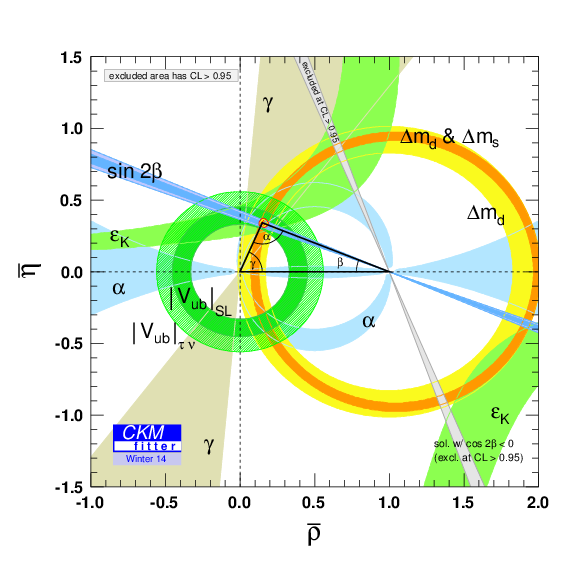
\includegraphics[scale=0.7]{rozdzial1/triangle.png}
 % Beetle_block.jpeg: 848x489 pixel, 96dpi, 22.44x12.94 cm, bb=0 0 636 367
 \caption{Przedziały dostępności kątów trójkąta unitarności (db) otrzymane w wyniku zebrania danych ze wszystkich eksperymentów.\cite{triangle} }
 \label{fig:trojkat wyniki}
\end{figure}


\subsection{Typy łamania symetrii \textbf{CP}}

Łamanie symetrii kombinowanej \textbf{CP} w ramach Modelu Standardowego, może zachodzić w trzech typach procesów.
\begin{itemize}
\item \textbf{Bezpośrednie łamanie symetrii \textbf{CP}} zwane również łamaniem w rozpadzie, zachodzi gdy występuje różnica pomiędzy częstościami rozpadów wzajemnie do siebie sprzężonych procesów. Zjawisko, to może się pojawiać zarówno dla naładowanych jak i neutralnych mezonów.
\item \textbf{Łamanie symetrii \textbf{CP} w mieszaniu} występuje tylko dla neutralnych mezonów, dla których to możliwa jest sytuacja gdzie stany własne masy nie są stanami własnymi oddziaływań słabych. W~ związku z~ powyższym faktem można zapisać posługując się notacją Dirca biorąc jak przykładowy mezon B:
\begin{eqnarray}
\ket{B_H}&=&p\ket{B^0}+q\ket{\overline{B^0}} \\ \nonumber
\ket{B_L}&=&p\ket{B^0}-q\ket{\overline{B^0}} 
\label{eq:Bh}
\end{eqnarray}
gdzie: stany po prawej stronie są stanami własnymi zapachu. natomiast te po lewej są stanami własnymi masy odpowiednio ciężkim $\ket{B_H}$ oraz lekkim $\ket{B_L}$. Warunek normalizacji wymaga aby w~ każdym momencie była spełniona zależność:
\begin{equation}
|q|^2+|p|^2=1
\label{eq:normalizacja}
\end{equation}
Ewolucja czasowa układu opisanego równaniem \ref{eq:Bh} reprezentowana jest zależnym od czasu równaniem Schrödingera. 
\begin{equation}
i\frac{d}{dt} \begin{pmatrix} p(t) \\ q(t)
\end{pmatrix}=\hat{\mathcal{H}} \begin{pmatrix} p(t) \\ q(t)
\end{pmatrix}=(\textbf{M}-\frac{i}{2}\Gamma) \begin{pmatrix} p(t) \\ q(t)
\end{pmatrix}
\label{Erwin}
\end{equation}
gdzie $\hat{\mathcal{H}}$- hamiltionian, $\textbf{M}$ oraz $\gamma$ są macierzami o~ rozmiarach 2x2. Pozadiagonalne elementy tych macierzy są odpowiedzialne za procesy mieszania. Zjawiska te można przedstawić w~ formie diagramów Feynmana, co zostało zrobione na rysunku \ref{rys:mixing}. W literaturze diagramy tego typu nazywane są diagramami pudełkowymi. 

 \begin{figure}[]
 \centering
 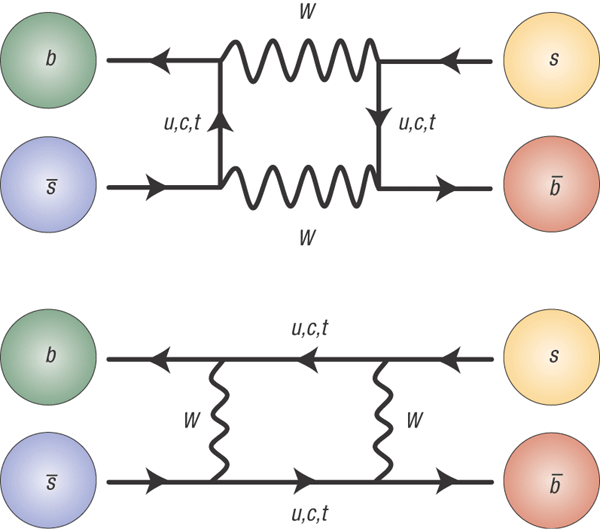
\includegraphics[scale=0.5]{rozdzial1/mixing.png}
 \caption{Diagramy Feynmana opisujące procesy mieszania neutralnych mezonów B. }
 \label{rys:mixing}
\end{figure}
  

Rozwiązanie krok po kroku równania \ref{Erwin} można znaleźć w~ \cite{nakada}. W~ niniejszej pracy przytoczone zostanie tylko ostateczny wynik.
\begin{equation}
\frac{p}{q} \propto \Delta M-\frac{i}{2}\Delta \Gamma
\label{pq}
\end{equation}

Łamanie symetrii \textbf{CP} zachodzi gdy $|\frac{p}{q}| \neq 1$. Analizując równanie \ref{pq} można wywnioskować, że aby znaleźć wielkość łamania symetrii kombinowanej \textbf{CP} należy bardzo dokładnie znać różnice w czasach życia oraz masach pomiędzy stanem ciężkim $\ket{B_H}$ oraz lekkim $\ket{B_L}$.

\item \textbf{Łamanie symetrii \textbf{CP} w interferencji pomiędzy rozpadem z mieszaniem i bez mieszania}\\
Zjawisko to jest związane z asymetrią pomiędzy rozpadami mezonów neutralnych zachodzącymi bezpośrednio $X^0\rightarrow f$ lub w wyniku mieszania $X^0\rightarrow \overline{X^0}\rightarrow f$. W takim wypadku stopień łamania symetrii jest proporcjonalny do części urojonej współczynnika $\eta_f$ opisanego zależnością \ref{eta}.
\begin{equation}
\eta_f =\frac{q}{p}\cdot \frac{A(\overline{X^0}\rightarrow f)}{A(X^0\rightarrow f)}
\label{eta}
\end{equation}

\end{itemize}

